\section{Graphen}
\subsection{s-t-Kanal Trennung}
\label{sub:app:st}
\begin{figure}[H]
    \begin{center}
        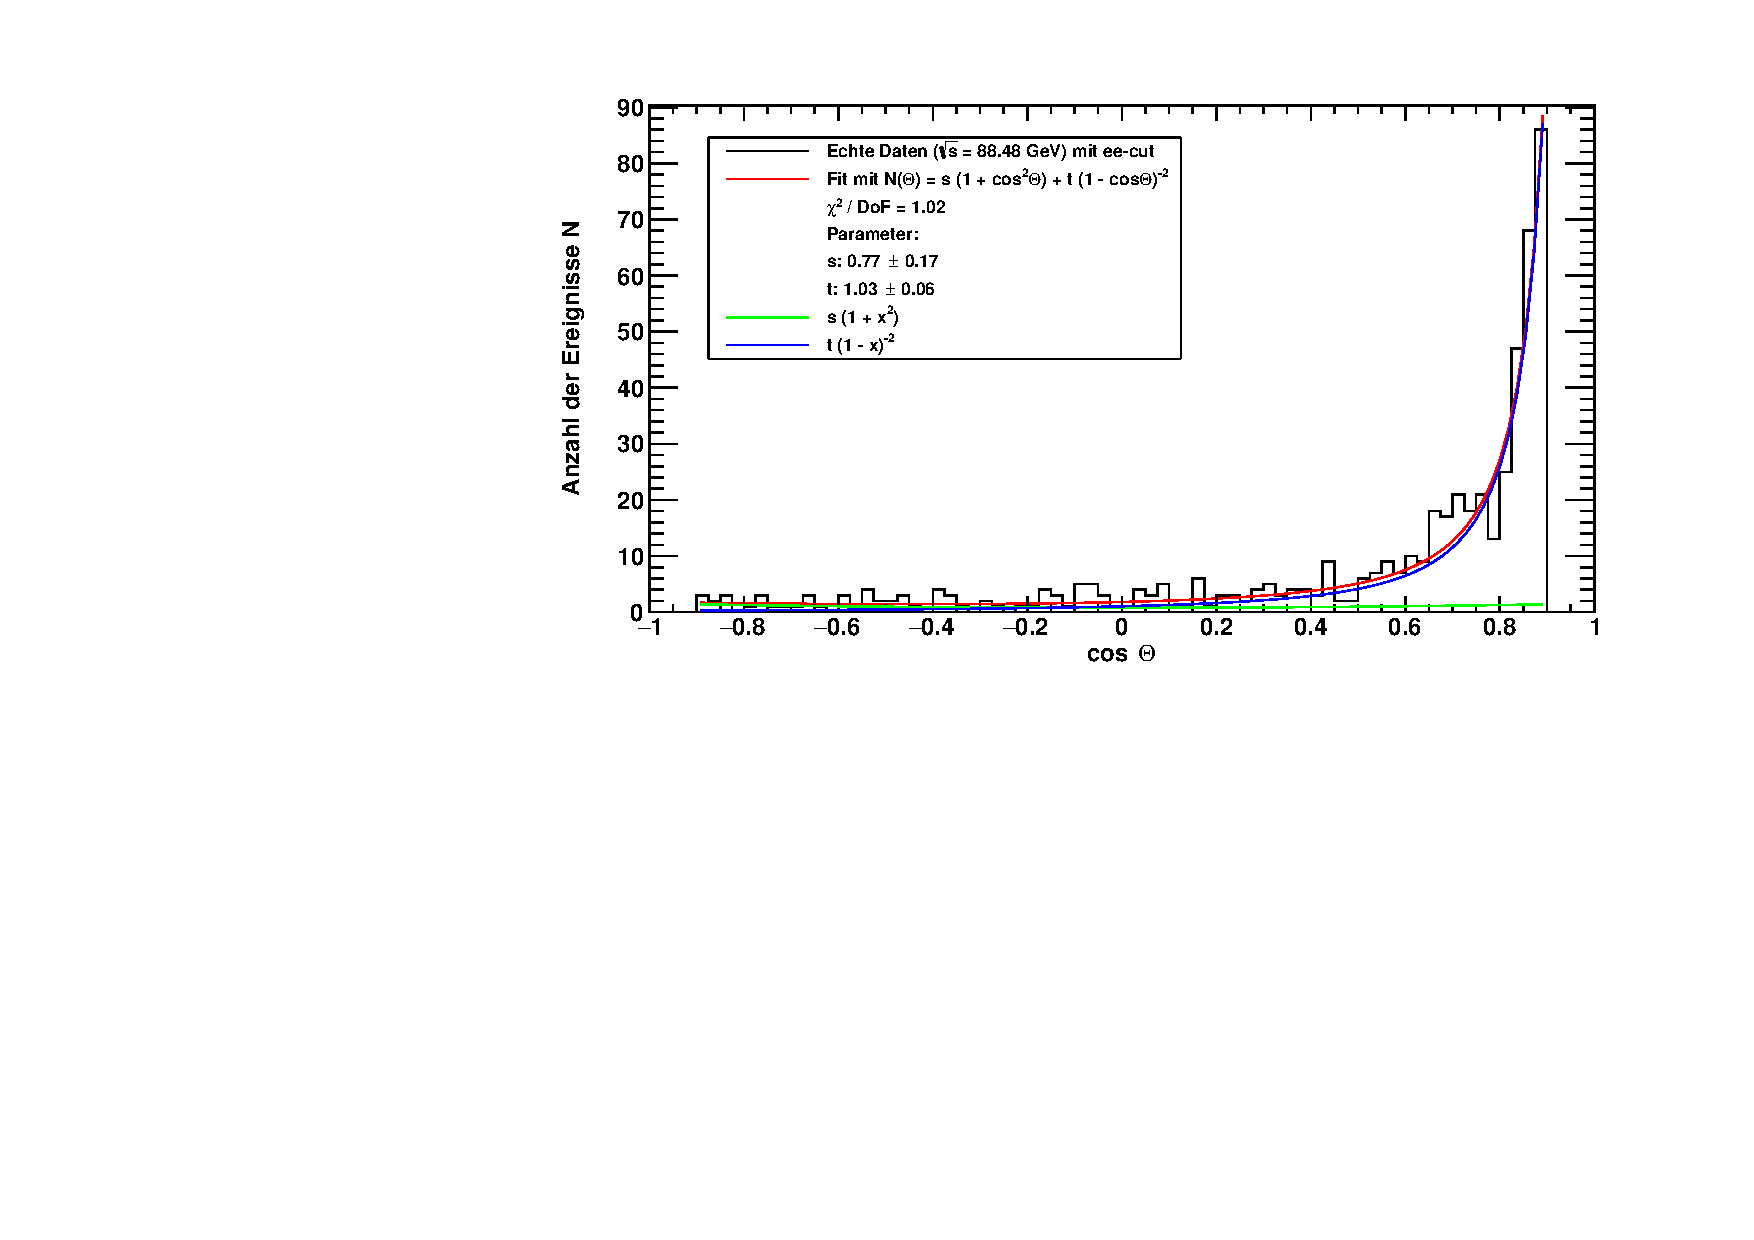
\includegraphics[width=\textwidth]{../img/s_t_fit_88-48.pdf}
        \caption{Winkelabhängigkeit der Ereignisse bei \sE{88.48} und Fit zur Bestimmung des s- und t-Anteils.}
        \label{img:st:8848}
    \end{center}
\end{figure}

\begin{figure}[H]
    \begin{center}
        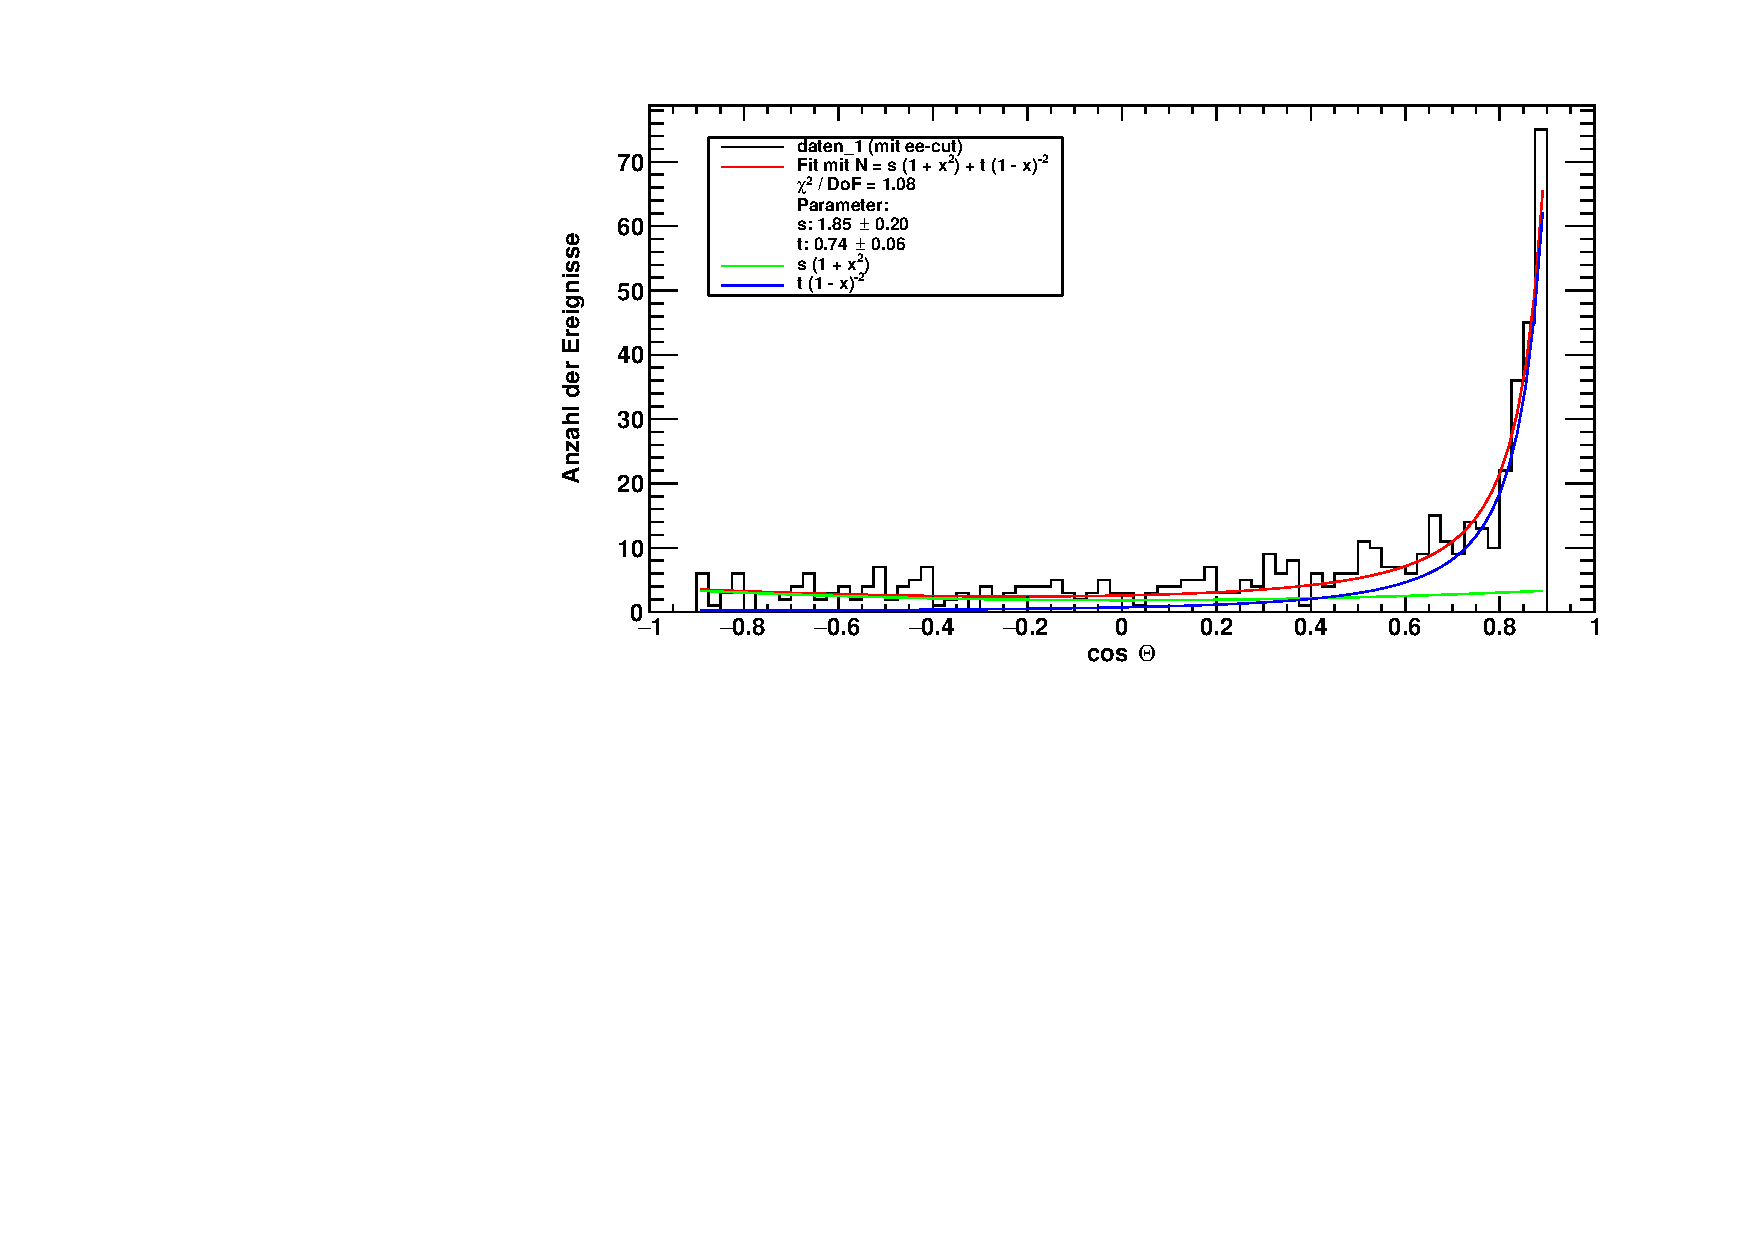
\includegraphics[width=\textwidth]{../img/s_t_fit_89-47.pdf}
        \caption{Winkelabhängigkeit der Ereignisse bei \sE{89.47} und Fit zur Bestimmung des s- und t-Anteils.}
        \label{img:st:8947}
    \end{center}
\end{figure}

\begin{figure}[H]
    \begin{center}
        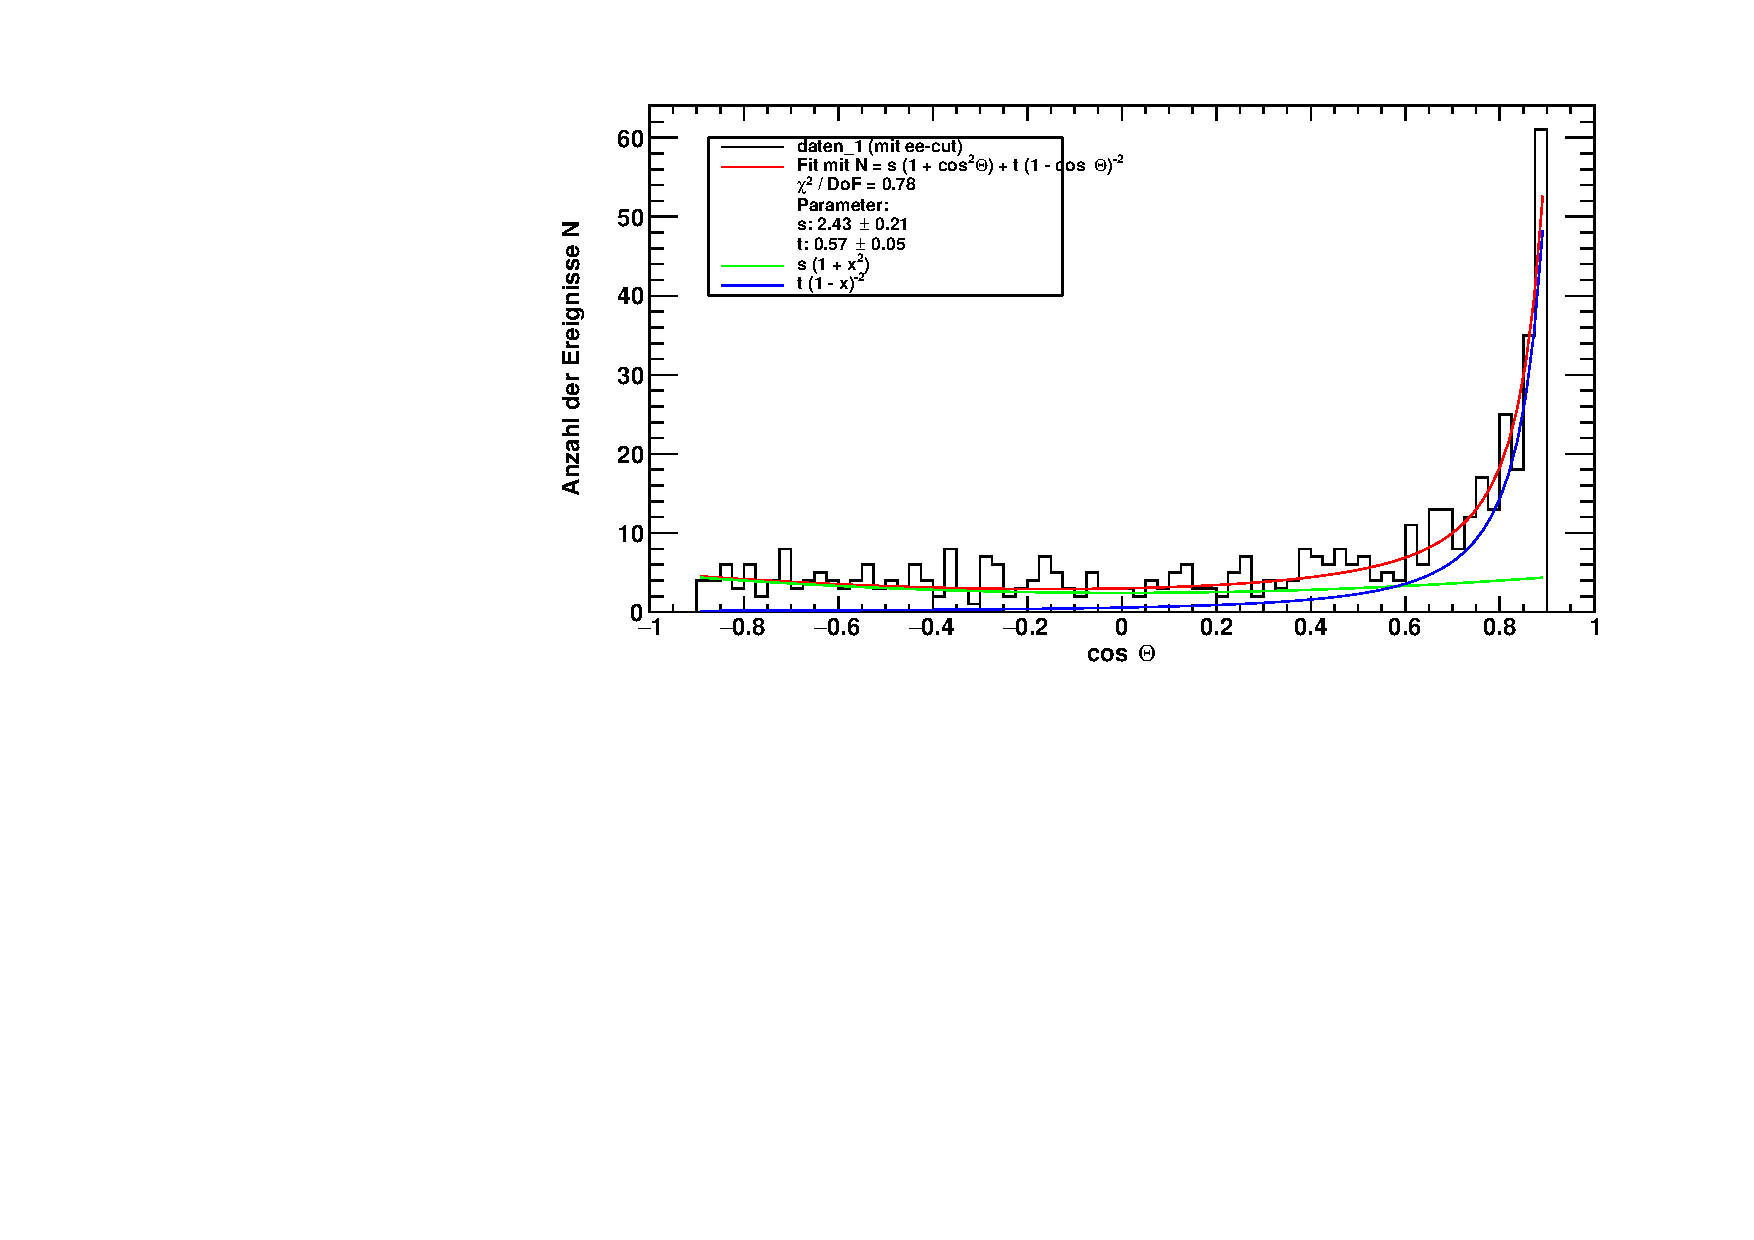
\includegraphics[width=\textwidth]{../img/s_t_fit_90-23.pdf}
        \caption{Winkelabhängigkeit der Ereignisse bei \sE{90.23} und Fit zur Bestimmung des s- und t-Anteils.}
        \label{img:st:9023}
    \end{center}
\end{figure}

\begin{figure}[H]
    \begin{center}
        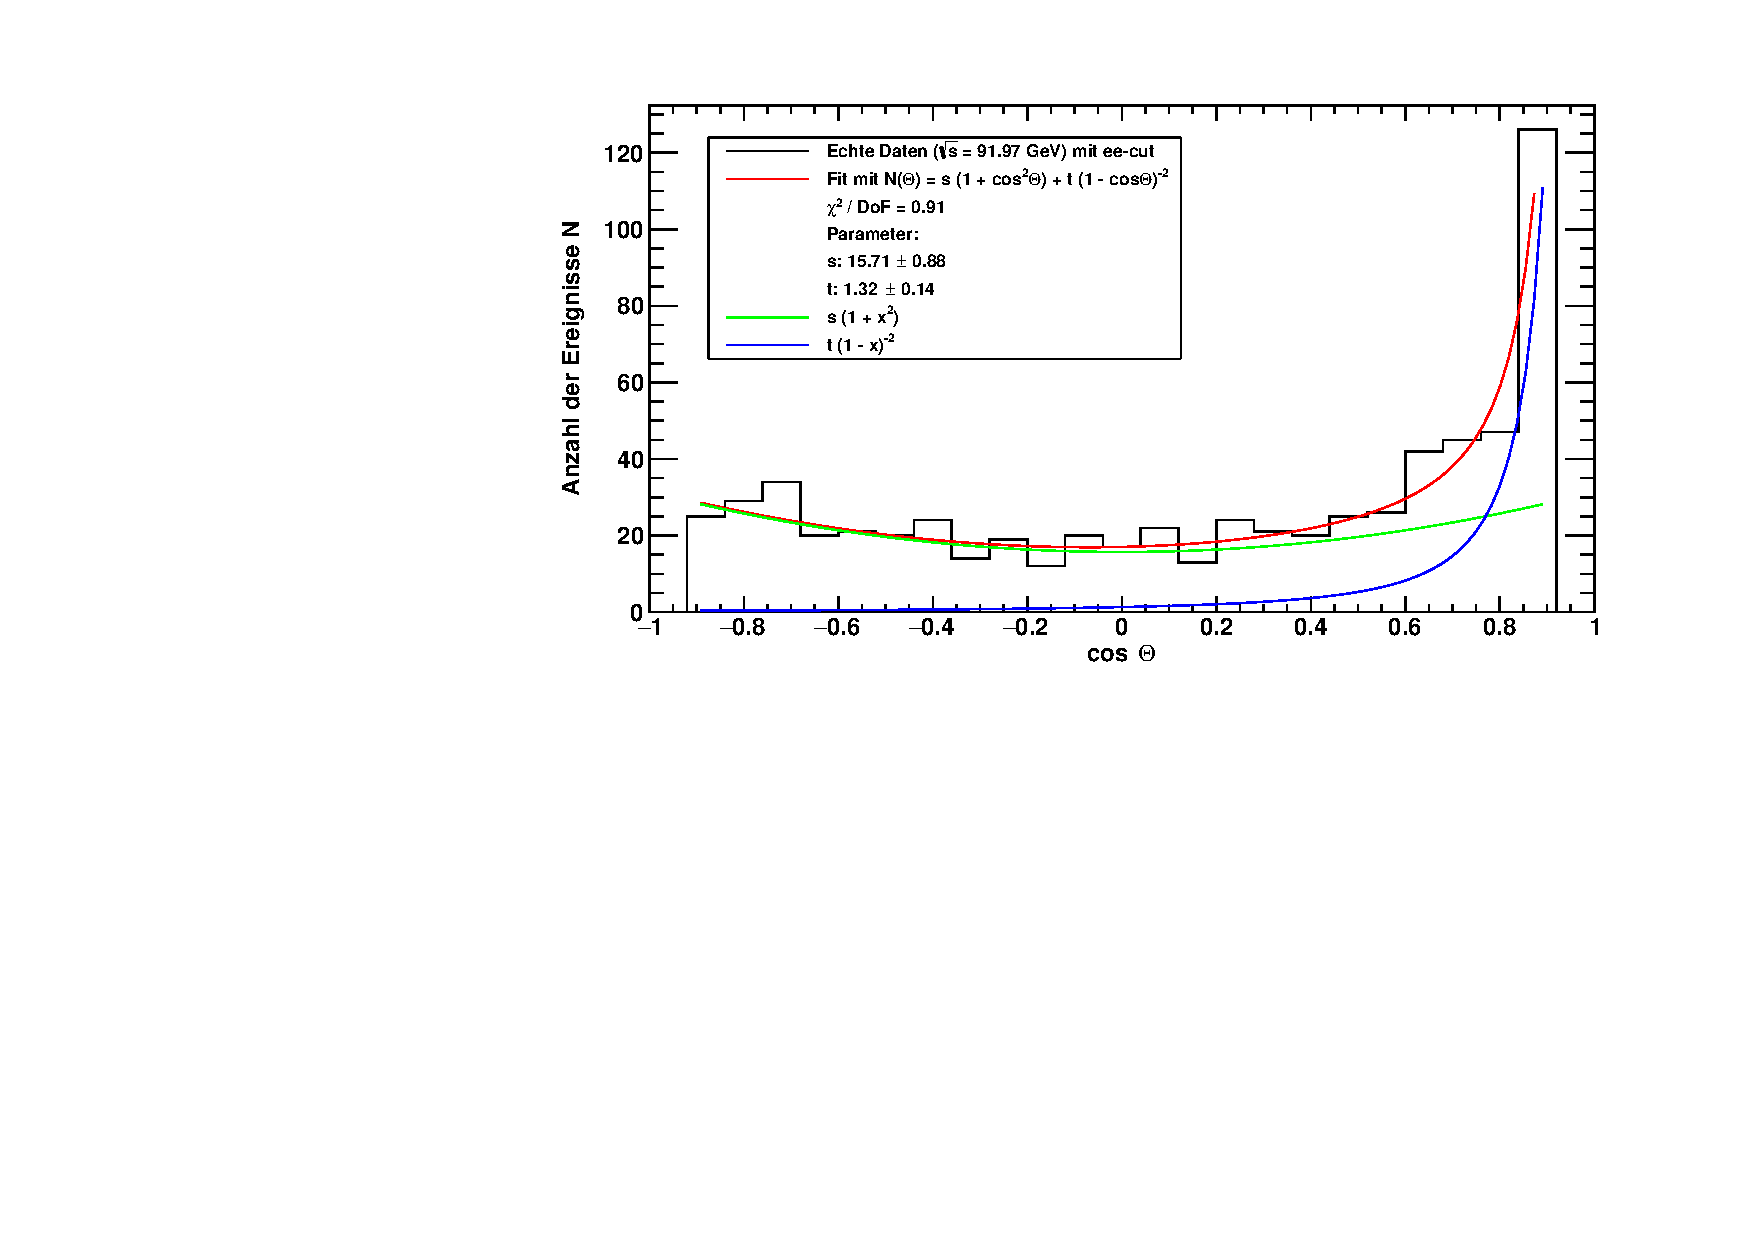
\includegraphics[width=\textwidth]{../img/s_t_fit_91-97.pdf}
        \caption{Winkelabhängigkeit der Ereignisse bei \sE{91.97} und Fit zur Bestimmung des s- und t-Anteils.}
        \label{img:st:9197}
    \end{center}
\end{figure}

\begin{figure}[H]
    \begin{center}
        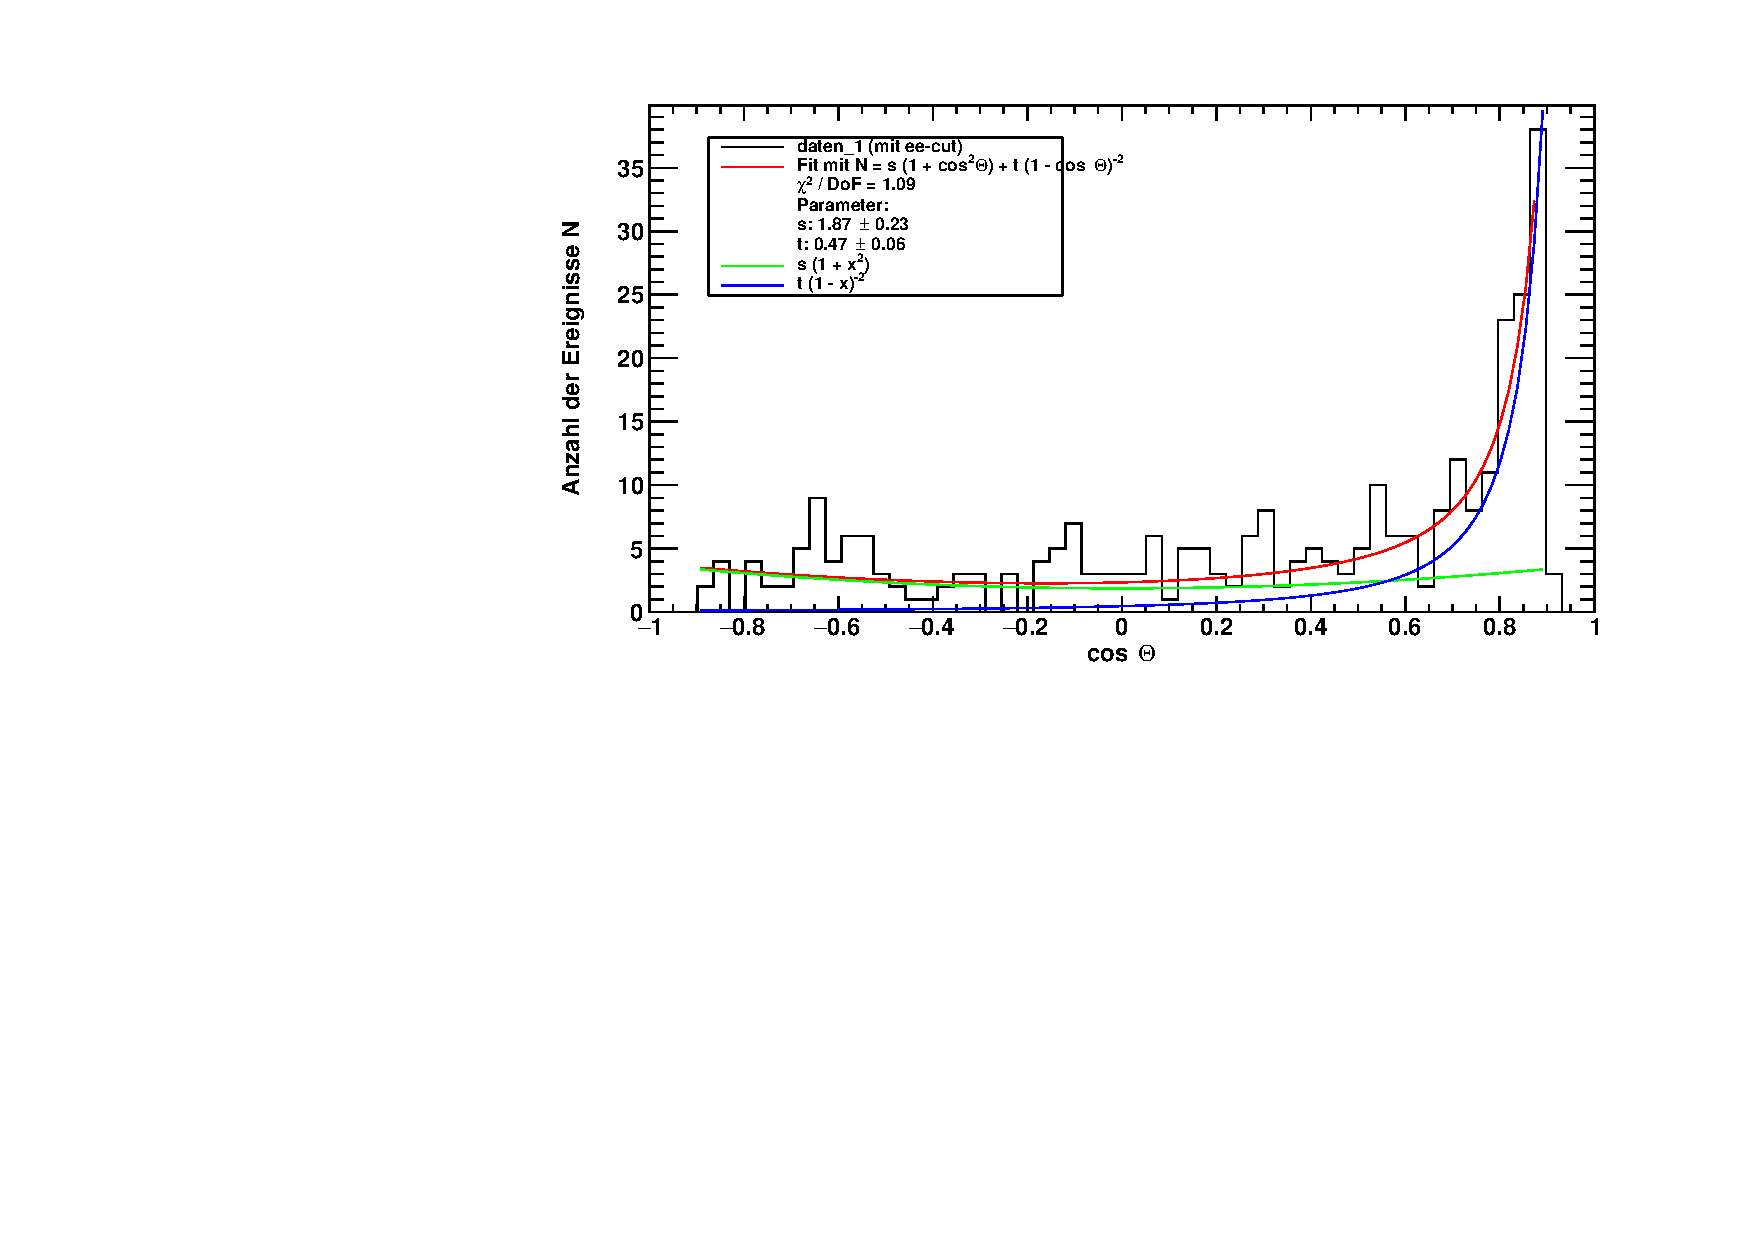
\includegraphics[width=\textwidth]{../img/s_t_fit_92-97.pdf}
        \caption{Winkelabhängigkeit der Ereignisse bei \sE{92.97} und Fit zur Bestimmung des s- und t-Anteils.}
        \label{img:st:9297}
    \end{center}
\end{figure}

\begin{figure}[H]
    \begin{center}
        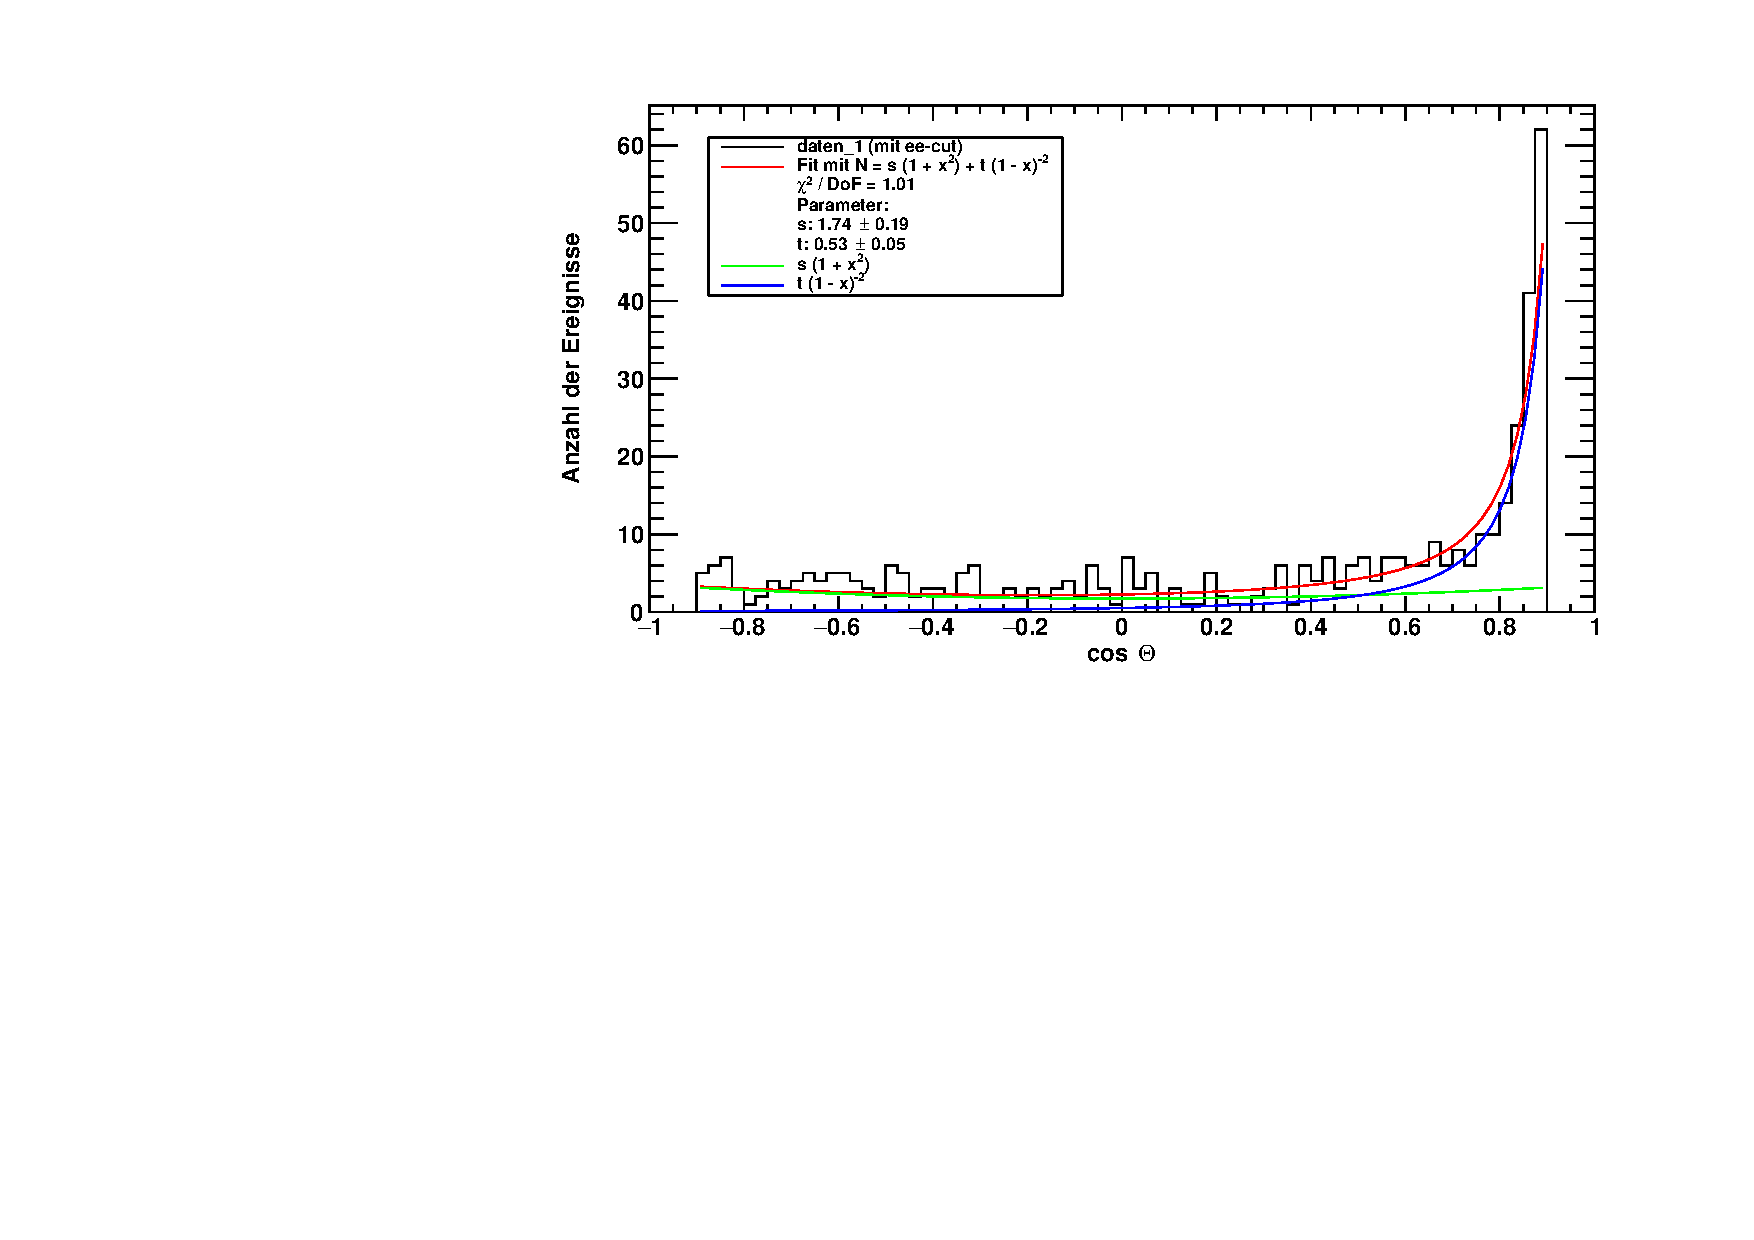
\includegraphics[width=\textwidth]{../img/s_t_fit_93-72.pdf}
        \caption{Winkelabhängigkeit der Ereignisse bei \sE{93.72} und Fit zur Bestimmung des s- und t-Anteils.}
        \label{img:st:9372}
    \end{center}
\end{figure}